\section*{Another study about the c variables}
In the past paper~\cite{Larkoski:2013eya}, It mention that in some process at $c_2$, when $\beta=1.7$, it will have the best separation power. We try to use this in our study to see whether it is suitable for our research.\\

In Figure 9,10 and 11, they are the ROC curves of the different $\beta$ quantities in $c_2$ at different energies of collision. We can see that in all cell sizes, separation power isn't improved by increasing $\beta$ quantity to 1.7. We can see from $\beta=1$ to $\beta=2$, the separation power is worse and worse in all cell sizes in all energies of collision.\\
\label{sec:c_variables_study}

%1$\times$1(cm$\times$cm)
\begin{figure}
\begin{center}
   \subfigure[5TeV] {
   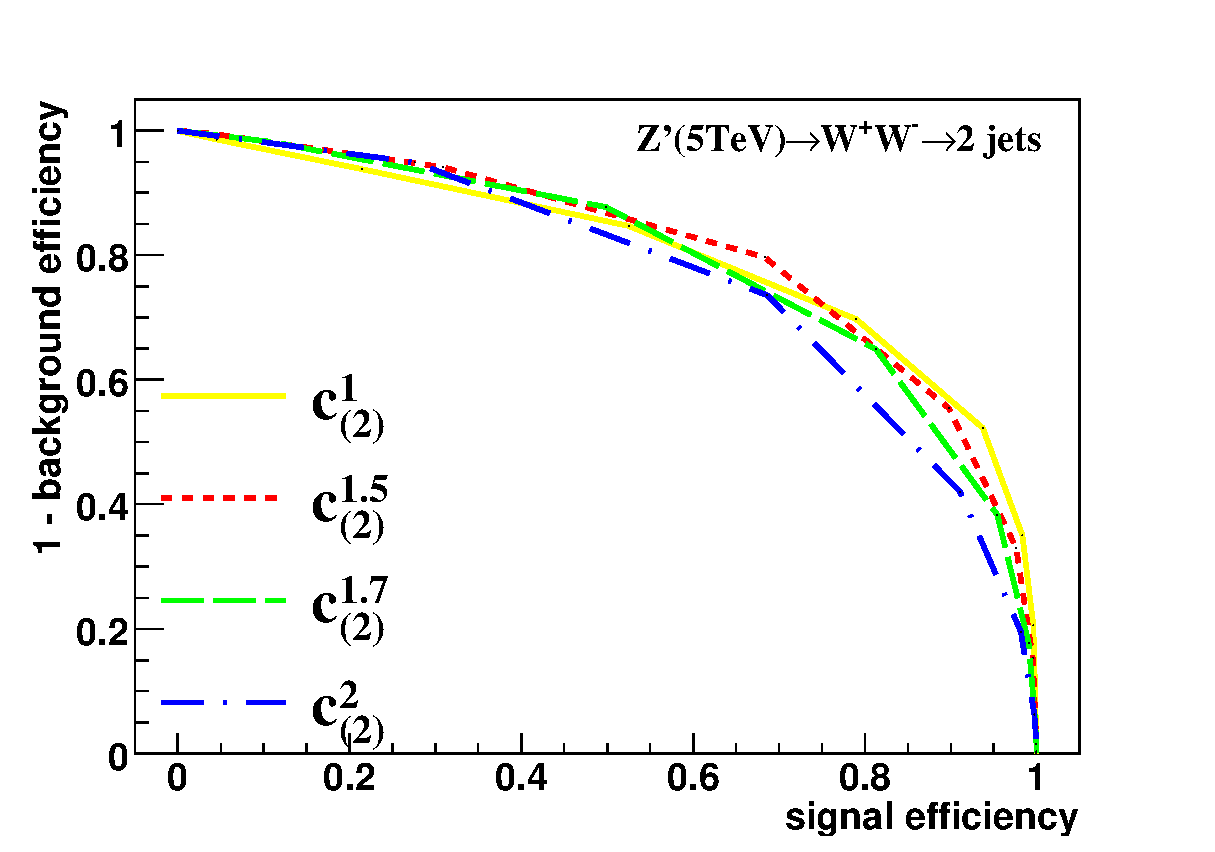
\includegraphics[width=0.43\textwidth]{figs/cluster_r010_c_variable_5tev_04_eff.eps}\hfill
   }
   \subfigure[10TeV] {
   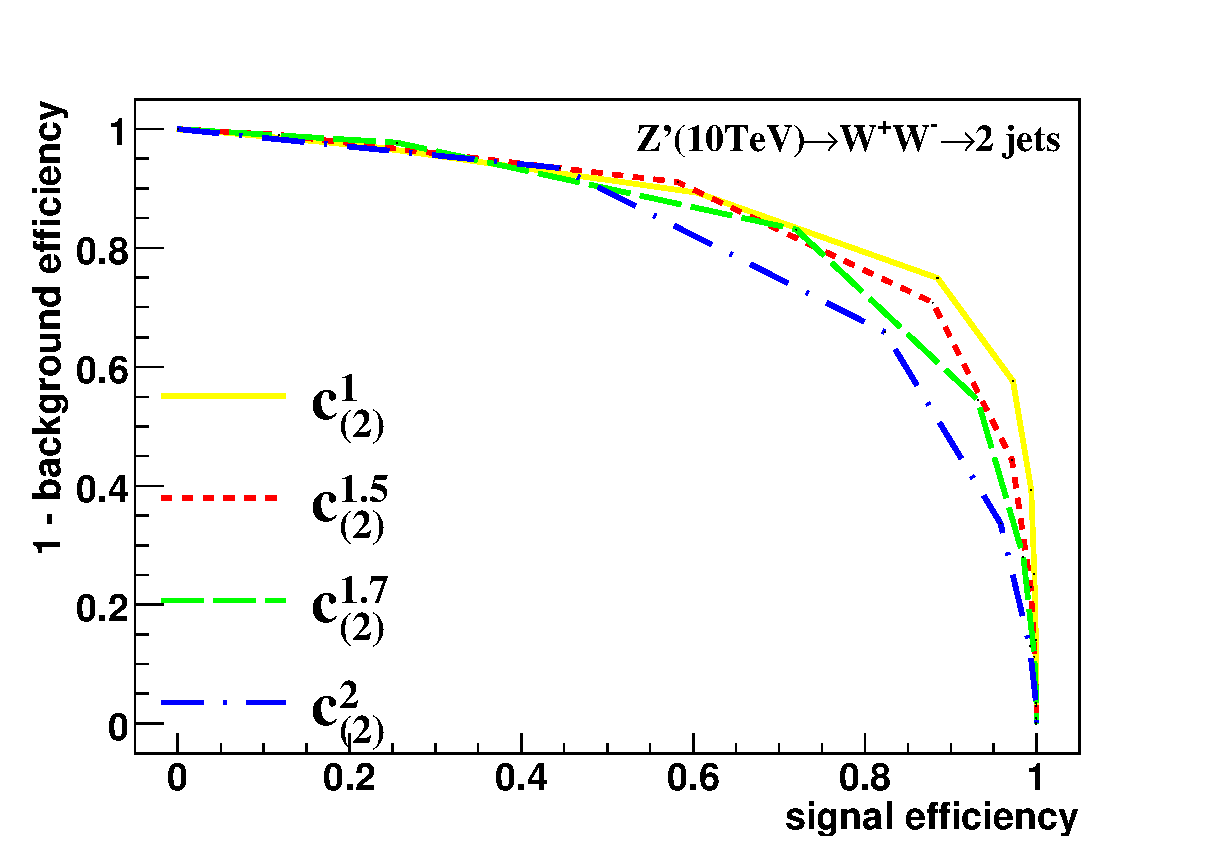
\includegraphics[width=0.43\textwidth]{figs/cluster_r010_c_variable_10tev_04_eff.eps}
   }
   \subfigure[20TeV] {
   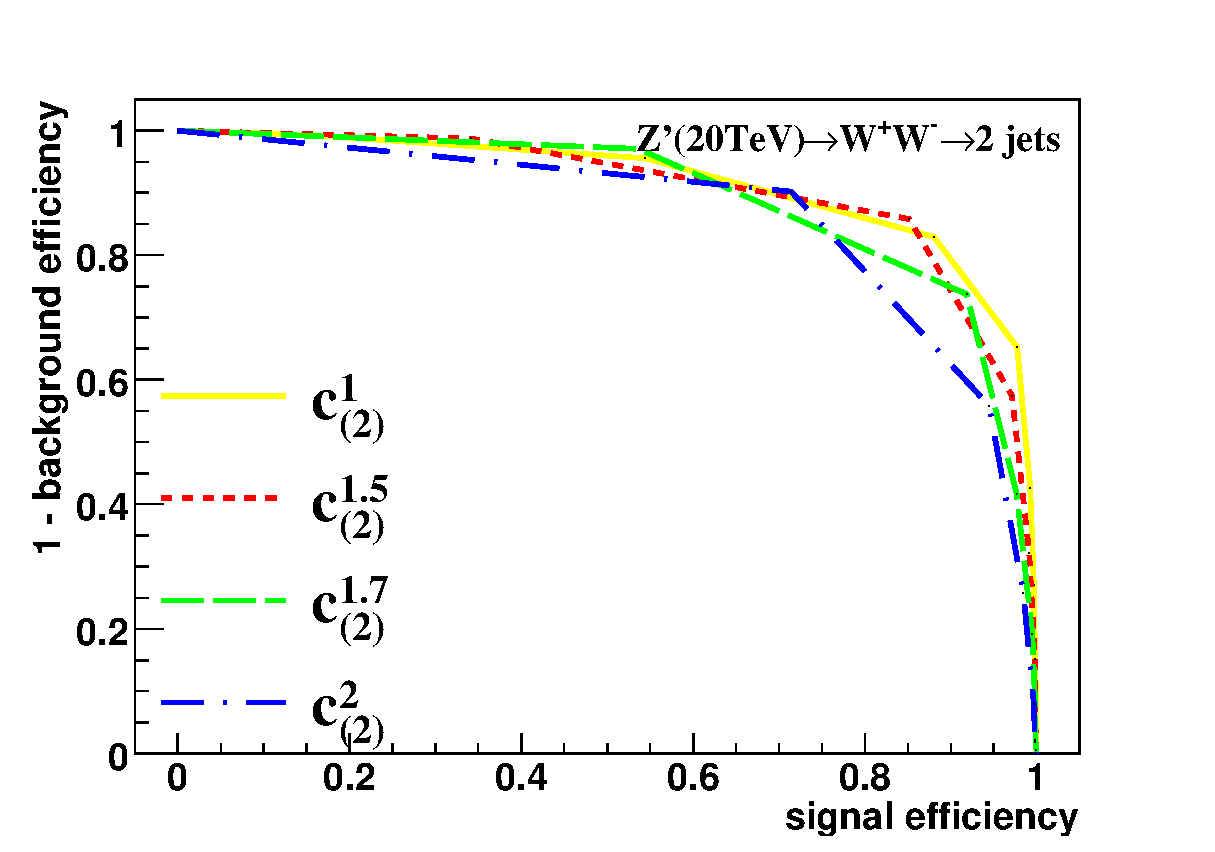
\includegraphics[width=0.43\textwidth]{figs/cluster_r010_c_variable_20tev_04_eff.eps}
   }
   \subfigure[40TeV] {
   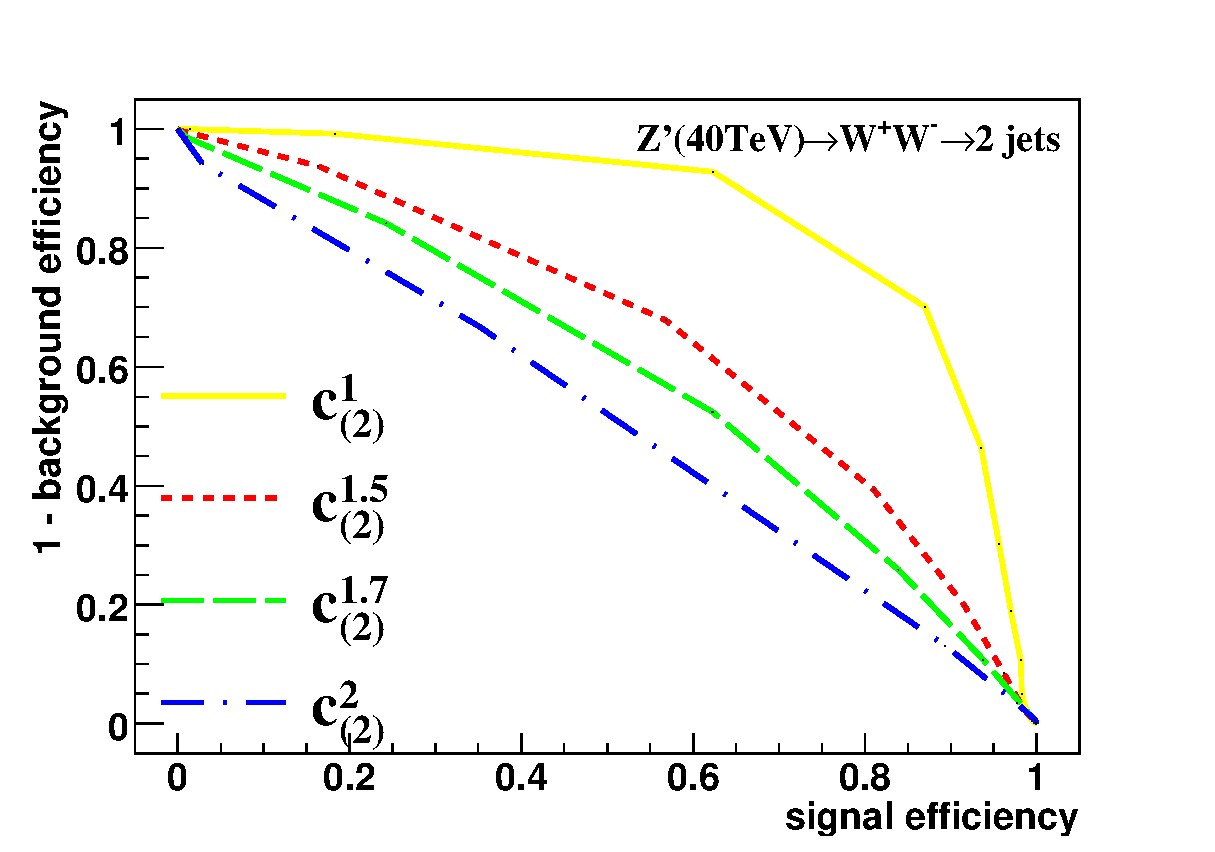
\includegraphics[width=0.43\textwidth]{figs/cluster_r010_c_variable_40tev_04_eff.eps}
   }

\end{center}
\caption{Signal efficiency versus background rejection rate using $c_2^{(1)}$,$c_2^{(1.5)}$,$c_2^{(1.7)}$,$c_2^{(2)}$ in different energies of collision at 20$\times$20(cm$\times$cm) cell size.The energies of collision at (a)5, (b)10, (c)20, (d)40TeV are shown here.}
\label{fig:cluster_r010_c_variable}
\end{figure}

\begin{figure}
\begin{center}
   \subfigure[5TeV] {
   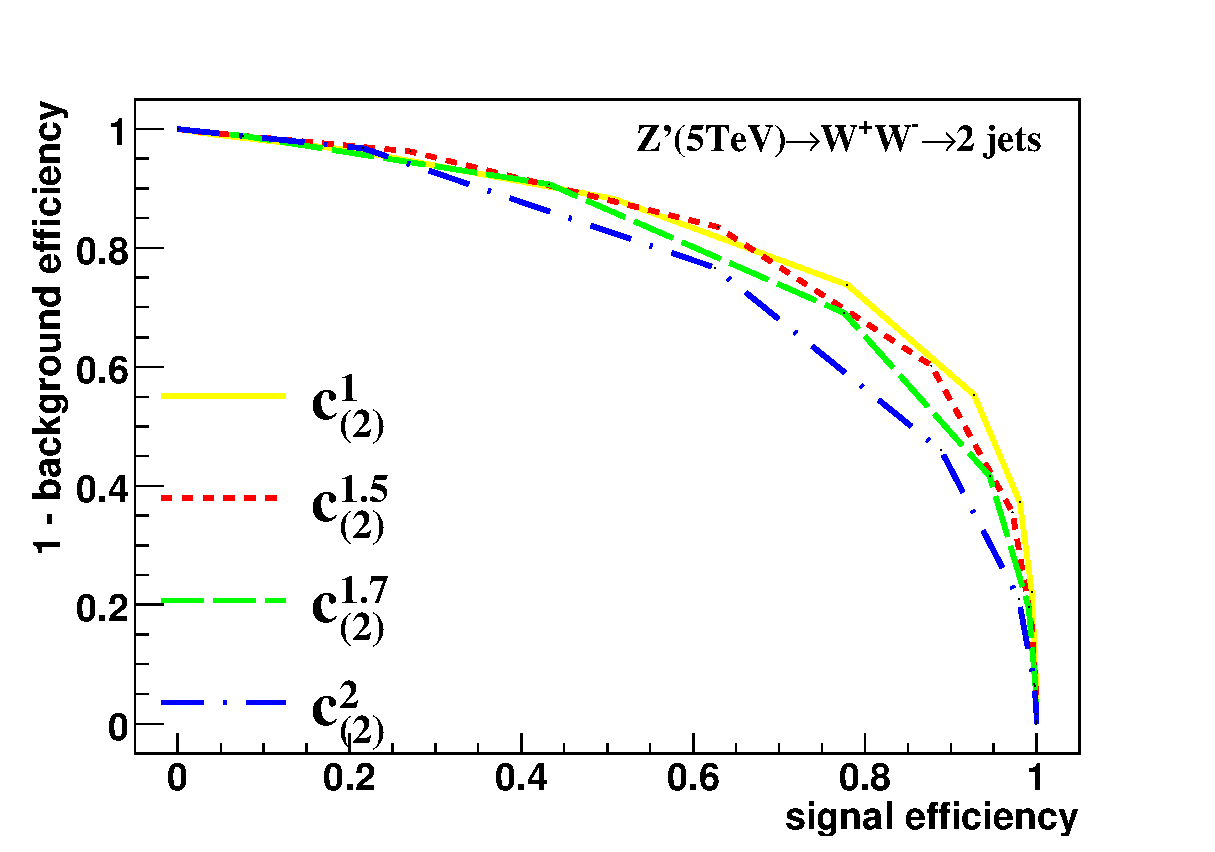
\includegraphics[width=0.43\textwidth]{figs/cluster_r009_c_variable_5tev_04_eff.eps}\hfill
   }
   \subfigure[10TeV] {
   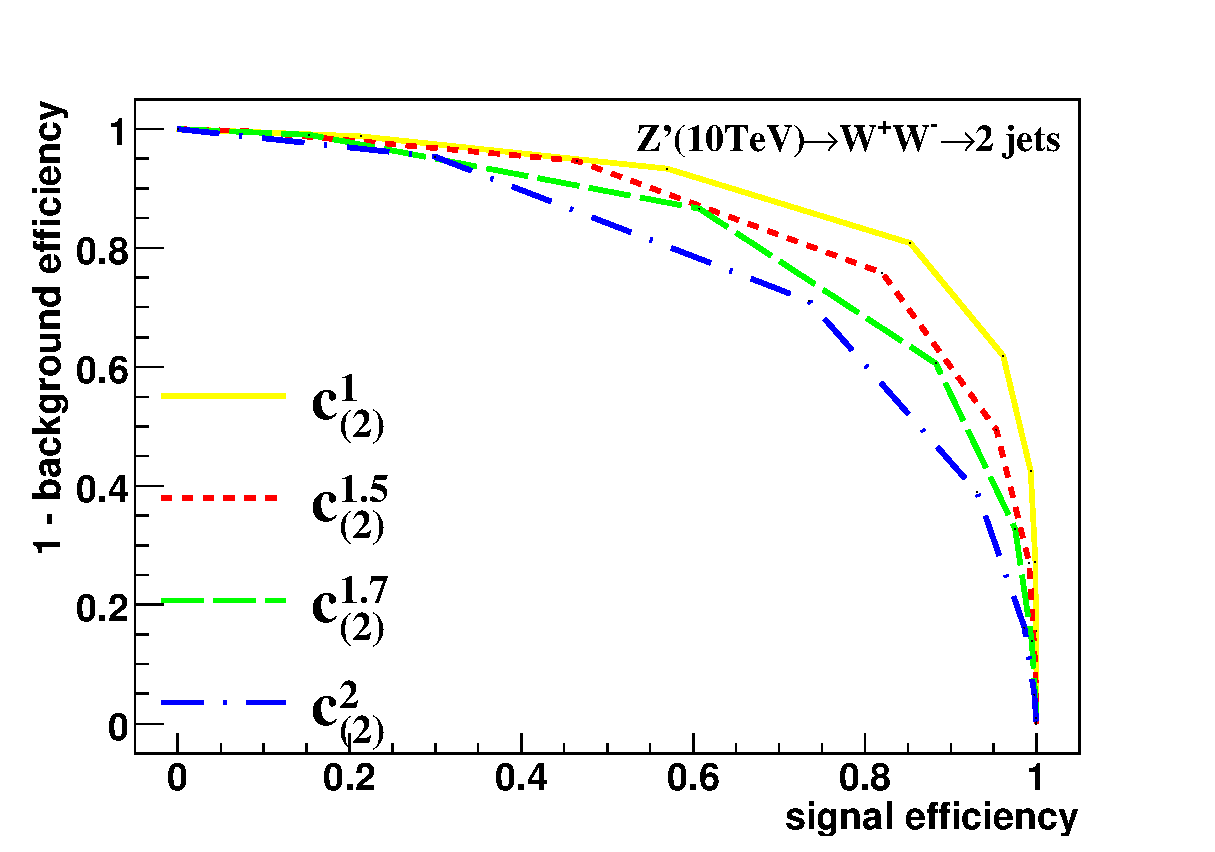
\includegraphics[width=0.43\textwidth]{figs/cluster_r009_c_variable_10tev_04_eff.eps}
   }
   \subfigure[20TeV] {
   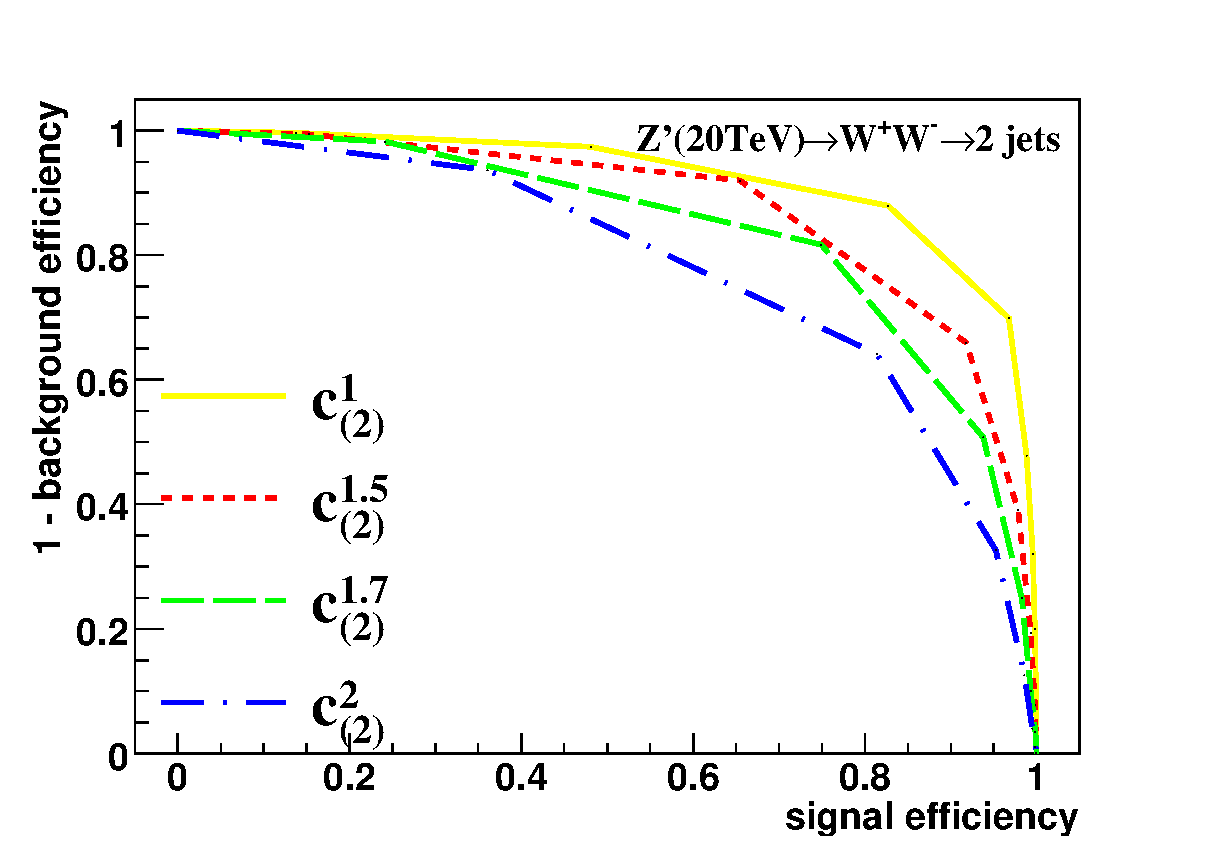
\includegraphics[width=0.43\textwidth]{figs/cluster_r009_c_variable_20tev_04_eff.eps}
   }
   \subfigure[40TeV] {
   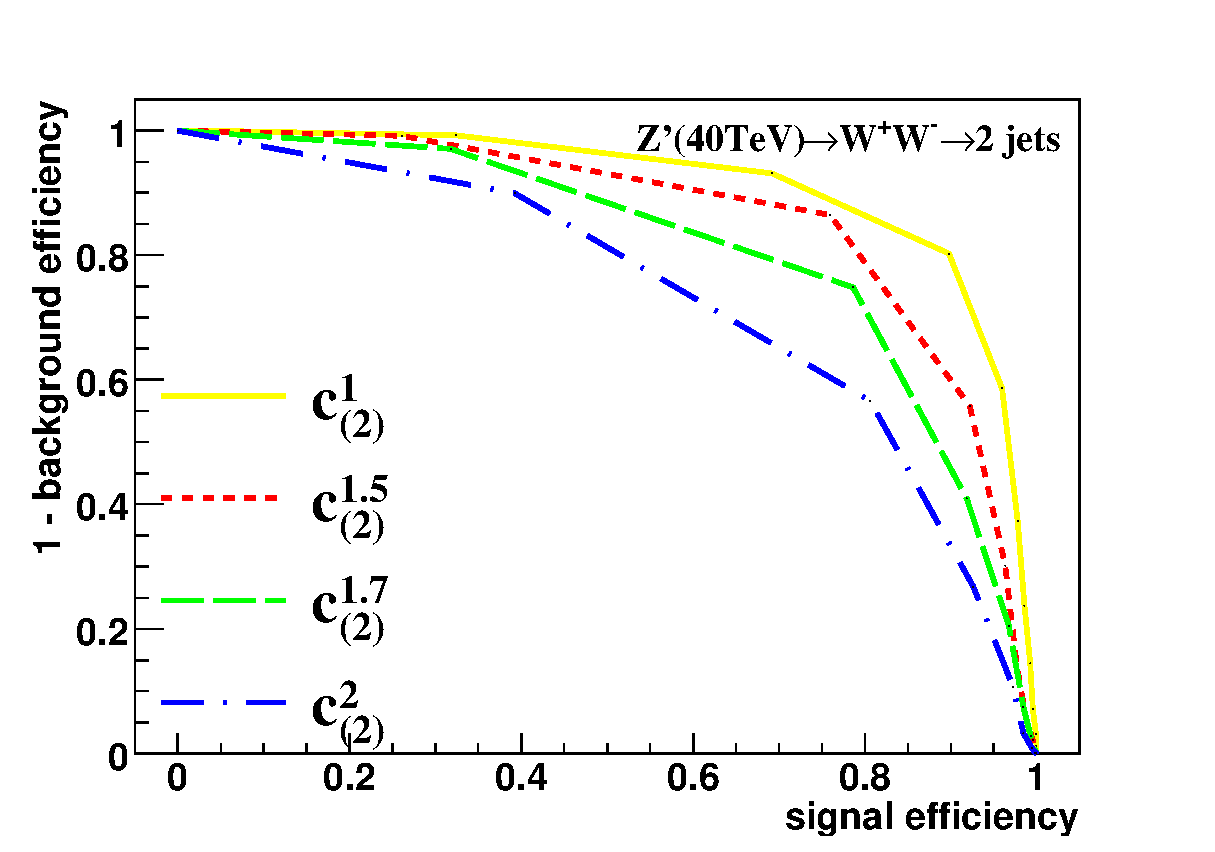
\includegraphics[width=0.43\textwidth]{figs/cluster_r009_c_variable_40tev_04_eff.eps}
   }

\end{center}
\caption{Signal efficiency versus background rejection rate using $c_2^{(1)}$,$c_2^{(1.5)}$,$c_2^{(1.7)}$,$c_2^{(2)}$ in different energies of collision at 5$\times$5(cm$\times$cm) cell size.The energies of collision at (a)5, (b)10, (c)20, (d)40TeV are shown here.}
\label{cluster_r009_c_variable}
\end{figure}

\begin{figure}
\begin{center}
   \subfigure[5TeV] {
   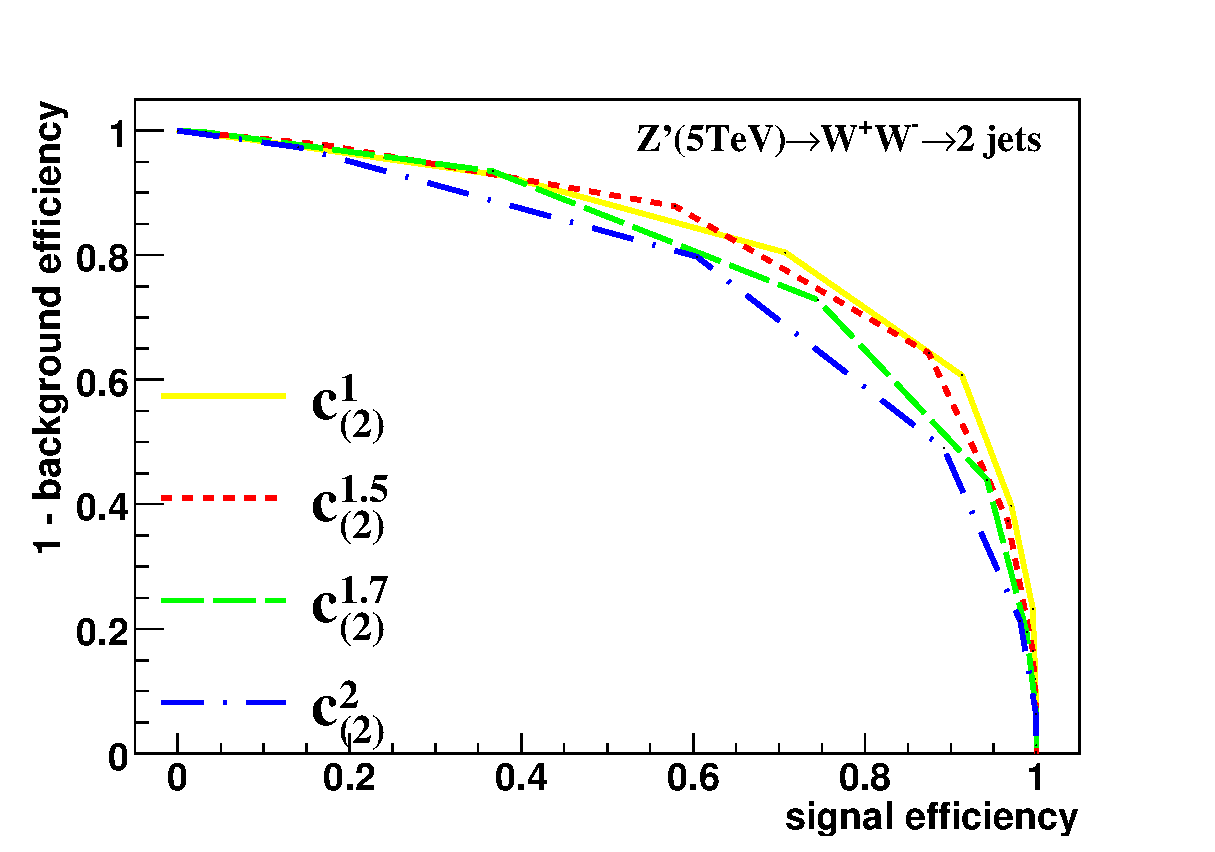
\includegraphics[width=0.43\textwidth]{figs/cluster_r012_c_variable_5tev_04_eff.eps}\hfill
   }
   \subfigure[10TeV] {
   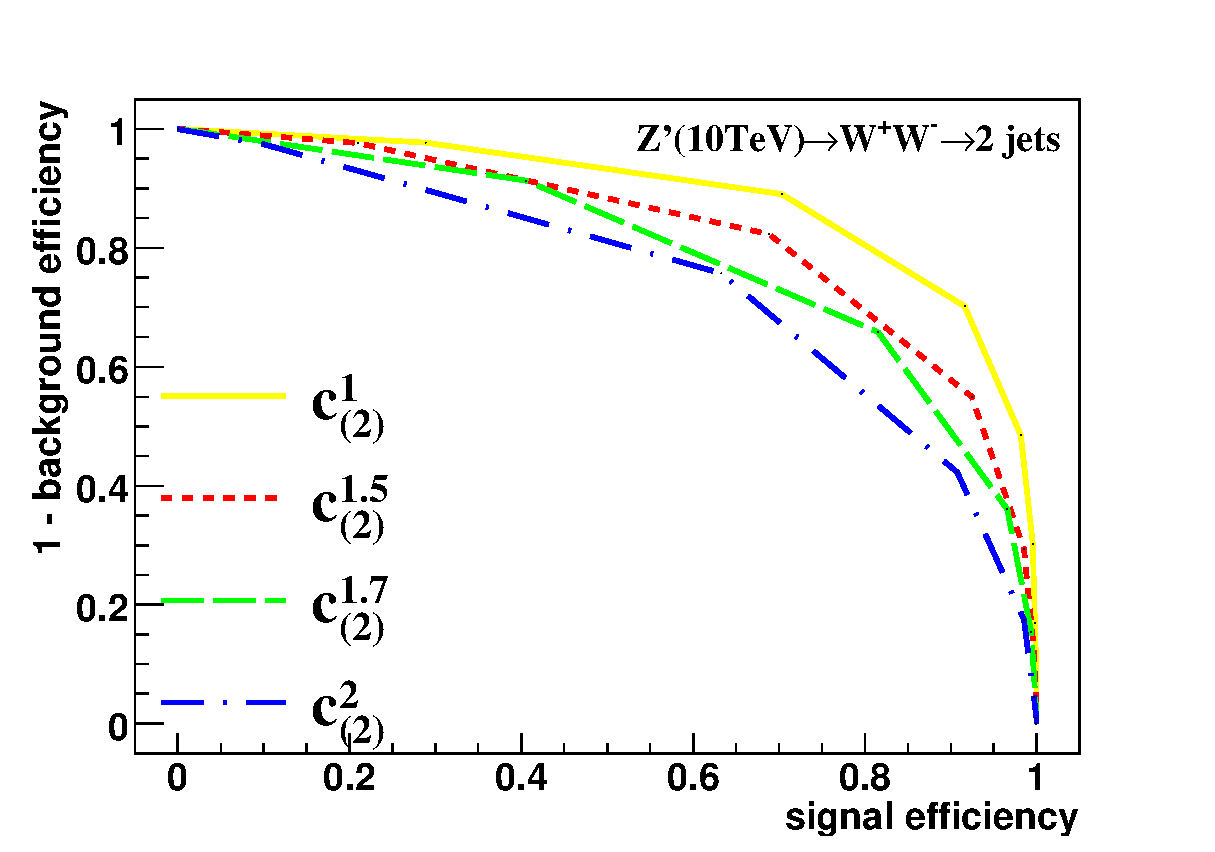
\includegraphics[width=0.43\textwidth]{figs/cluster_r012_c_variable_10tev_04_eff.eps}
   }
   \subfigure[20TeV] {
   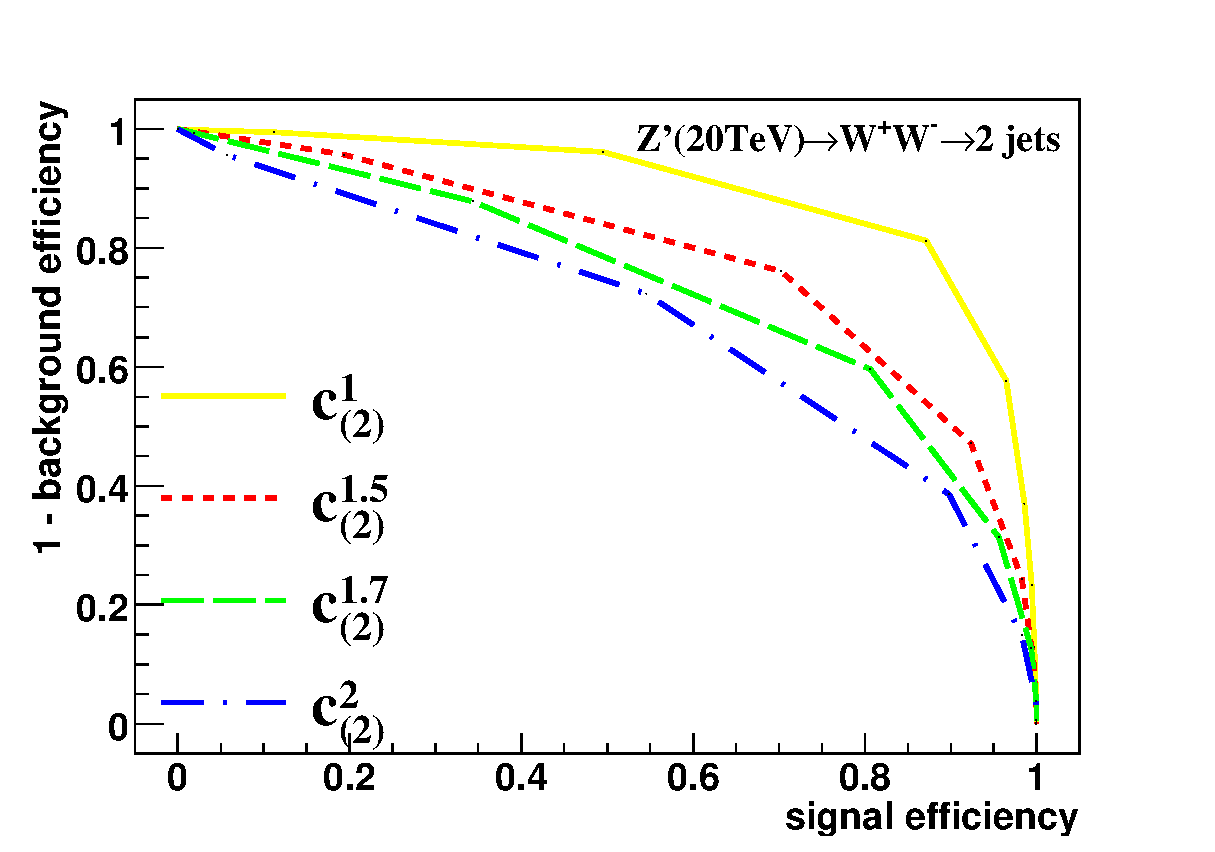
\includegraphics[width=0.43\textwidth]{figs/cluster_r012_c_variable_20tev_04_eff.eps}
   }
   \subfigure[40TeV] {
   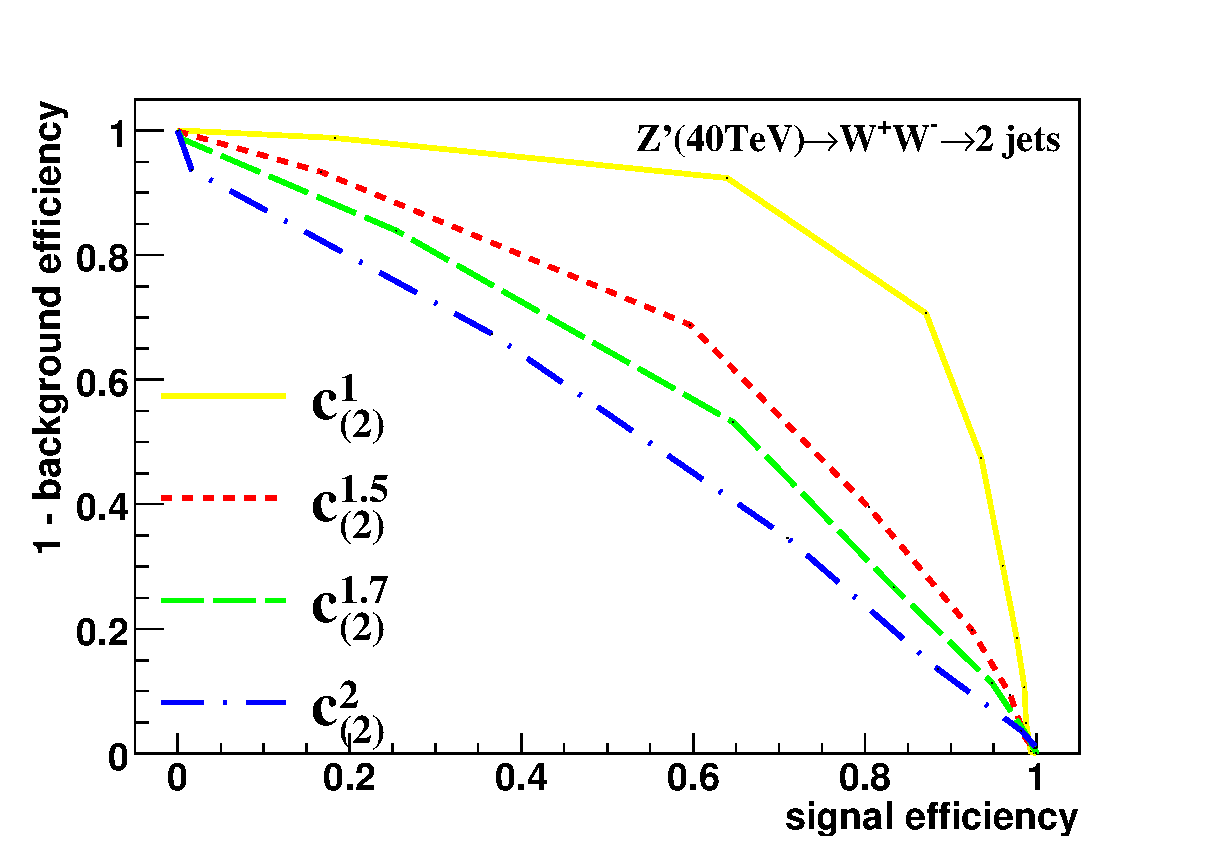
\includegraphics[width=0.43\textwidth]{figs/cluster_r012_c_variable_40tev_04_eff.eps}
   }

\end{center}
\caption{Signal efficiency versus background rejection rate using $c_2^{(1)}$,$c_2^{(1.5)}$,$c_2^{(1.7)}$,$c_2^{(2)}$ in different energies of collision at 1$\times$1(cm$\times$cm) cell size.The energies of collision at (a)5, (b)10, (c)20, (d)40TeV are shown here.}
\label{cluster_r012_c_variable}
\end{figure}


